\chapter{Tecniche di caratterizzazione dei workload}
I workload reali sono la migliore opzione per andare a valutare le performance specifiche di un dato sistema, il problema è che mantenere tale workload richiede un ingente quantità di memoria. Quindi è nata la necessità di trovare e ricercare delle tecniche che permettessero di poter caratterizzare un workload reale e ridurre la quantità di dati da memorizzare per poterne avere una statistica quanto meno affidabile

\section{Terminologia}
Gli argomenti che saranno affrontati durante tale capitolo richiedono una conoscenza della specifica terminologia utilizzata. In generale i concetti fondamentali da conoscere inerenti al dispositivo ed al componente da testare sono:
\begin{itemize}
    \item \textbf{DUT}(Device Under Test): Sistema che viene sottoposto ad uno specifico test (es. CPU o un processo di transazione)
    \item \textbf{CUT}(Component Under Test): Componente del sistema di cui si vogliono conoscere le performance (es.ALU o Unità Disco)
    \item \textbf{Metrica}: Metrica che si vuole andare a valutare per il CUT (es. MIPS o T/s)
\end{itemize}

\begin{figure}[h]
\centering
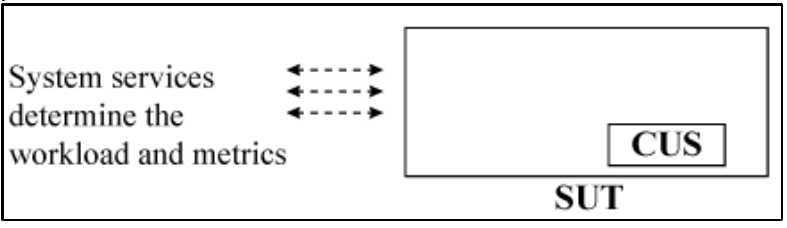
\includegraphics[width=.8\textwidth]{img/chapter-3/CUS-SUT.png}
\caption{Struttura del sistema di test}\label{img:cus-sut}
\end{figure}

Oltre la terminologia intrinseca al sistema di test bisogna definire anche la terminologia inerente ad altre entità interagenti. Quindi si definiscono i seguenti termini:
\begin{itemize}
    \item \textbf{User}: entità che esegue le richieste di servizio
    \item \textbf{Workload components}(Qualitative identifiers): Componenti basilari che mi permettono di capire a livello qualitativo cosa fa un workload, quindi la natura e la struttura delle attività che vengono svolte dalle varie componenti (es. transazione in un database, una query in un motore di ricerca o Un processo o thread in un sistema operativo)
    \item \textbf{Workload parameters}(Quantitative Identifiers): Sono parametri quantitativi associati al workload e che quindi descrivono come le componenti si comportano. Servono principalmente per avere una misura numerica delle caratteristiche del workload (es. Arrival rate [Quante richieste al secondo], il service time [quanto tempo serve per completare un compito], Resource Usage [quante risorse vengono consumate], I/O operations [quante lettura/scritture su disco avvengono])
\end{itemize}

\section{Workload Characterization Tecniques}
\begin{info}
La \textbf{Workload Characterization} è un processo che permette di definire un workload di test di dimensione ridotta, ma che conservi tutte le caratteristiche e le proprietà (sia statiche che dinamiche), del workload reale. Ciò ne permette la replicazione e l'utilizzo in ambito di performance analysis.
\end{info}
C'è però da capire come sia possibile estrarre il workload sintetico dal workload reale, pertanto sono state utilizzare e definite diverse tecniche negli anni. L'obbiettivo principale di tali tecniche è quello di trovare dei parametri ridotti con cui cercare di poter descrivere il workload reale a meno di una certa quantità di informazione persa (tale quantità saraà valutata in vari modi, solitamente si utilizzerà la varianza o la devianza).

\subsection{Averaging}
La tecnica dell'\textbf{Averaging} è molto semplice, cerca di ridurre il workload in una singola istanza i cui parametri vengono valutati con la media dei parametri presenti nel workload reale. Quindi quello che si va a fare è:
\\
Siano: \({x_1,x_2, \dots, x_n}\) i valori assunti nel workload dal parametro \(x\), allora si può approssimare tale parametro tramite la media aritmetica definita come:
\[
\overline{x} = \frac{1}{n}\sum_{i=1}^{n}x_i
\]
Talvolta però non è proprio l'ideale utilizzare la media, ciò dipende fortemente dalla tipologia di dati che si ha. Solitamente si potrebbe pensare di utilizzare altre tecniche come: la mediana (permette di prendere un valore appartenente al workload più centrale), oppure il 50-percentile, la media geometrica ecc.

\subsubsection{Specifying Dispersion}
Caratterizzare un workload reale mediante un workload sintetico prevede di avere, intrinsecamente, degli errori. Ciò accade principalmente per la limitatezza che ho nei parametri che voglio andare a considerare (non posso avere memoria di tutte le istanze del workload reale, ma solo di alcune di esse).
Si potrebbe pensare di andare a stimare l'errore mediante la somma di tutte le deviazioni, ovvero:
\[
errore\_totale = \sum_{i=1}^{n}(x_i-\overline{x})
\]
Tale rappresentazione, però, non è proprio utile, il problema principale risiede nel segno che possono avere le deviazioni (immaginiamo il caso di avere 5 e 15, la media è 10, ma l'errore, se calcolato con la formula sopra è 0 [(5-10) + (15-10)]), il che porta a rendere tale ragionamento errato.
Un'altra soluzione potrebbe essere quella di andare a considerare la deianza, ovvero la somma degli errori quadratici
\[
errore\_totale = \sum_{i=1}^{n}(x_1 - \overline{x})^2
\]

La devianza, quindi, risolve il problema del segno delle deviazioni, ma dipende fortemente dal numero di dati.
Data quindi tale dipendenza dal numero di dati della devianza, si preferisce utilizzare la \textbf{varianza campionaria}, che va a dividere la devianza per n - 1. Si va a considerare n - 1 per  via dei gradi di libertà, ovvero, il numero di deviazioni linearmente indipendenti [warning successivo]
\[
s^2 = \frac{1}{n-1}\sum_{i=1}^{n}(x_i-\overline{x})^2
\]

\begin{warn}

\textit{Tale dimostrazione non è stata fatta in aula, per quanto sia semplice non è richiesta ai fini dell'esame ma solo per questione di conoscenza personale.}\\ 
Tale formula ci fa capire perchè dividiamo per n-1 nella varianza capionaria e perchè tale divisione è giustificata come il numero di \textbf{gradi di libertà}
\[
\sum_{i=1}^{n}(x_i - \overline{x}) = \sum_{i=1}^{n}x_i - \sum_{i=1}^{n}\overline{x} = \sum_{i=1}^{n}x_i - \overline{x} \sum_{i=1}^{n}1 = \sum_{i=1}^{n}x_i - n \overline{x} = 
\]
\[
=\sum_{i=1}^{n}x_i - n \left(\frac{1}{n}\sum_{i=1}^{n}x_i\right) =\sum_{x=1}^{n}x_i - \sum_{x=1}^{n}x_i = 0
\]

Dopo tale dimostrazione si comprende che le devianze linearmente indipendenti sono n-1, dato che una sarà esprimibile come somma delle altre
\end{warn}

Oltre al concetto di varianza, solitamente, si preferisce parlare di deviazione standard, dato che è espressa nell'unità di misura della grandezza che si sta andando a valutare. La deviazione standard si calcola come radice quadrata della varianza campionaria, ovvero:
\[
s = \sqrt{s^2}
\]

Oltre a tale valore, per rendersi conto dell'incertezza rispetto ai dati effettivi (essere in grado di confrontare un sistema piccolo con un sistema grande cercando di evitare un confronto rispetto alle grandezze di misura), è utile considerare il \textbf{coefficente di variazione}, che viene definito come:
\[
COV = \frac{s}{\overline{x}}
\]

Un esempio di utilizzo di tale valore è il seguente:
Immaginiamo di avere due sistemi e di averne valutato il tempo di risposta e la deviazione standard associata ad ogni sistema. Si avrà il seguente scenario:
\begin{itemize}
    \item \textbf{Sistema 1}: response time = 10 ms, dev. standard = 2 ms
    \item \textbf{Sistema 2}: response time = 200 ms, dev. standard = 15 ms
\end{itemize}

Se mi chiedessi quale dei due sistemi risulta più \textbf{stabile}, allora intuitivamente andrei a confrontare le dev. standard e valuterei quella minore come più stabile. Ma questo, però, non viene messo a confronto con gli andamenti medi (non guardo la larghezza della campana rispetto alla sua altezza [gaussiana]). Pertanto se calcolo i coefficenti di variazione, avrò che per il sistema 1: COV = 0,2 = 20\%; mentre per il sistema 2: COV = 0,075 = 7,5\%. Il che mi dimostra che il sistema 2 è più stabile rispetto al sistema 1 (completamente il contrario rispetto alla decisione iniziale).

\subsection{Single Parameter Histogram}
Il \textbf{Single Parameter Histogram} si occupa di costruire un istogramma delle occorrenze che vada a caratterizzare il \textbf{singolo parametro} considerato ed analizzato. La costruzione di un istogramma viene effettuata andando a valutare la frequenza di occorrenza di un dato valore in base ad una sua distribuzione discreta. 

Più formalmente quello che si va a costruire è una funzione \(f(x)\) che mi dice quante volte il parametro \(x\) assume un certo valore. Tale funzione viene costruita andando a suddividere l'intervallo di valori che il parametro può assumere in \textbf{buckets} (o bins), ovvero sottointervalli. Quindi si va a contare quante volte il parametro assume un valore compreso in un certo bucket e si va a riportare tale conteggio sull'asse delle ordinate, mentre sull'asse delle ascisse si riporta il bucket considerato.

Vi sono però dei problemi nell'utilizzare tale tecnica, utilizzare un istogramma per ogni parametro vuol dire utilizzare grandi quantità di memoria, a livello numerico:
Consideriamo \(n \)bucket  per ogni valore (intervalli di cui si deve tenere traccia), \(m\) il numero di parametri per ogni componente, ed \(k\) il numero di componenti, allora la memoria richiesta per memorizzare tale istogramma sarà:
\[
Memoria = n m k
\]

Ciò risulta troppo dettagliato per la reppresentazione del workload, oltretutto, tale metodo non tiene conto delle correlazioni tra i vari parametri, dato che ogni istogramma viene costruito in maniera indipendente dagli altri, ciò porta quindi a portare all'interno della descrizione del workload anche parametri che potrebbero essere deducibili da altri (ridondanza di informazioni). Questo pregiuduca anche la possibilità di selezionare i parametri da considerare mediante la varianza, dato che dati che non sono indipendenti porterebbero la stessa quantità di informazione.

\subsection{Multiparameter Histogram}
Il \textbf{Multiparameter Histogram} è una tecnica che cerca di risolvere i problemi del single parameter histogram, andando a considerare le correlazioni tra i vari parametri. Quello che si va a fare è costruire un istogramma che consideri non swolo le frequenze di un singolo parametro, ma le frequenze di n-parametri, correlate tra di loro. Per comprendere la complessità nella costruzione di un istogramma a n-variabili, vediamo un esempio con due variabili, che sarebbe quello mostrato in figura [\ref{img:multi-histograms}]. Per leggere tale grafico dobbiamo considerare 3 assi, che nel nostro caso sono rappresentati come:
\begin{itemize}
    \item \textbf{Asse X}: rappresenta il range di valori del primo parametro
    \item \textbf{Asse Y}: rappresenta il range di valori del secondo parametro
    \item \textbf{Asse Z}: Viene rappresentato mediante la griglia quadrettata, ed il valore considerato è il numero di punti che sono presenti per un dato intreccio di valori.
\end{itemize}

Ciò ci aiuta a capire come si possono trovare dei pattern tra i vari parametri, data la specifica distribuzione dei parametri (in questo caso le due variabili crescono l'una rispetto all'altra). La problematica principale risiede nella quantità di parametri che bisognerebbe incatenare per trovare delle correlazioni tra le variabili, ed oltretutto, per workload molto grandi risulta complicato andare a memorizzare tale quantità di dati anche andando a considerare un filtro con la varianza.

\begin{figure}[h]
\centering

\begin{subfigure}[b]{0.8\textwidth}
\centering
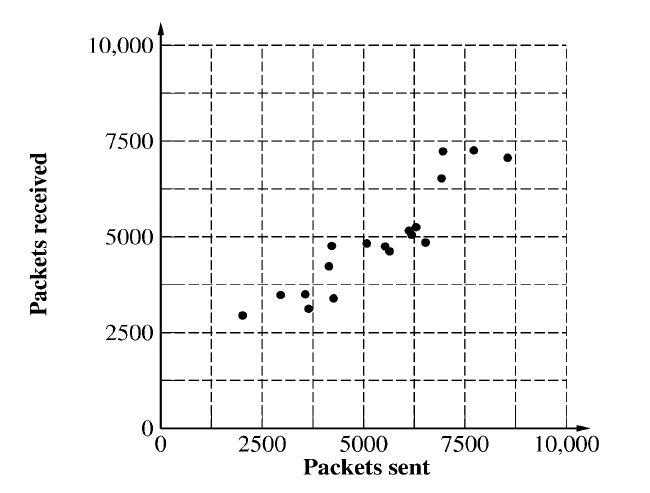
\includegraphics[width=\textwidth]{img/chapter-3/multi-histogram.png}
\caption{Multiparameter Histogram on 2D space}\label{img:multi-histogram}
\end{subfigure}

\hfill

\begin{subfigure}[b]{0.8\textwidth}
\centering
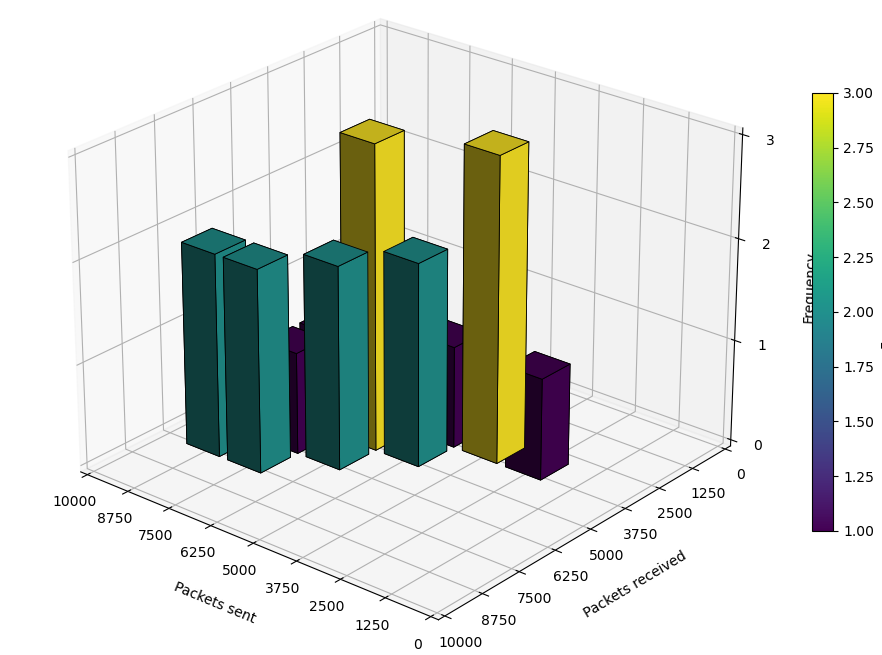
\includegraphics[width=.8\textwidth]{img/chapter-3/multi-histogram-3d.png}
\caption{Multiparameter Histogram on 3D space}
\label{img:multi-histogram-3d}
\end{subfigure}

\caption{Esempi di istogrammi multiparametrici}\label{fig:multi-histograms}
\end{figure}

\clearpage
\subsection{Principal Component Analysis (PCA)}
Un modo utilizzato per ridurre il numero di parametri con cui andare a rappresentare le istanze del workload è la \textbf{Principal Component Analysis (PCA)}. Tale tecnica ha come compito quello di trasformare l'insieme di istanze in altre istanze, le nuove istanze vengono definite sulla base delle componenti principali (che differiscono dai parametri reali), poichè nel nuovo spazio, tali parametri sono tutti linearmente indipendenti, e non ci sono correlazioni. Il funzionamento matematico della PCA è basato sull'effettuazione di una media pesata per ogni parametro. Precisamente:
\\
Dati i parametri \({x_1,x_2,\dots,x_N}\), si vuole trovare un nuovo insieme di parametri \({y_1,y_2,\dots,y_N}\), voglio però che l'insieme di parametri \(y_i\) sia linearmente indipendente, e che la varianza di ogni parametro \(y_i\) sia massimizzata. Di base per vedere come andare a costruire la matrice di trasformazione della PCA, si dovrebbe calcolare la matrice di covarianza, una volta calcolata si valutano gli autovettori di tale matrice, che costruiranno poi la matrice di trasformazione finale. Gli autovettori, quindi, rappresentano le direzioni principali e sono disposti in maniera che la prima componente principale sia quella con la varianza maggiore. Difatto si sta andando a fare una media pesata dei parametri per costruire il valore della nuova componente principale. Precisamente:
\[
y_j = \sum_{i=1}^{N}w_{ij}x_{ij}
\]

Tale formula va letta in questo modo:
\begin{itemize}
    \item \textbf{\(y_j\)}: rappresenta la j-esima componente principale
    \item \textbf{\(x_{ij}\)}: rappresenta il valore del parametro \(i\) nell'istanza \(j\)
    \item \textbf{\(w_{ij}\)}: rappresenta il peso associato al parametro \(i\) per la j-esima istanza
\end{itemize}

Per effettuare la PCA bisogna seguire i seguenti passi:
\begin{enumerate}
    \item Andare a calcolare la matrice di covarianza dei dati (prima si potrebbero effettuare anche operazioni di normalizzazione)
    \item Andare a calcolare gli autovettori e gli autovalori della matrice di covarianza
    \item Costruire la matrice di trasformazione mediante gli autovettori ordinati secondo gli autovalori in maniera decrescente (gli autovalori portano con loro la quantità di varianza, quindi ordinando gli autovettori si avrà uno spazio in cui il primo parametro copre la maggior varianza [utile per la selezione di un minor numero di parametri])
\end{enumerate}

In maniera più compatta, quindi, effettuata la PCA, si avrà che:
\begin{itemize}
    \item I nuovi parametri y sono calcolabili come combinazioni lineari dei parametri x
    \item I parametri y sono linearmente indipendenti, dato che il prodotto interno tra due parametri y è 0
    \item Il nuovo set di parametri y è ordinato in maniera tale che la varianza del primo parametro è maggiore della varianza del secondo e così via
\end{itemize}

\subsubsection{Z-Score Normalization}
La \textbf{z-score normalization} è una tecnica che permette di andare a normalizzare i dati, in maniera tale che ogni parametro abbia media 0 e deviazione standard 1. Tale tecnica è utile per poter effettuare la PCA, dato che si vuole evitare che parametri con range di valori molto diversi tra di loro possano influenzare in maniera sproporzionata il risultato finale. La formula per effettuare tale normalizzazione è la seguente:
\[
x'_s = \frac{x_{s} - \overline{x_s}}{s_{x_s}}
\]

Tale operazione permette di poter confrontare i parametri con un distribuzione normale, il che, quindi, andrà a rappresentare i dati come distanza da 0 e rappresentato secondo la deviazione standard s. Ciò ci permette anche di poter confrontare i dati tra di loro, senza andarea a considerare il range di valori che possono assumere.

\subsection{Clustering}
Mediante l'utilizzo della PCA si è andata ad effettuare la riduzione della quantità di parametri rappresentativi di un istanza (o componente) del workload. Per ridurre ancora di più la quantità di dati di rappresentazione del workload, si può andare ad effettuare una riduzione della quantità di istanze stesse. Per effettuare tale riduzione si fa utilizzo del \textbf{Clustering}, che è una tecnica di apprendimento non supervisionato che permette di andare a raggruppare le istanze in base alla loro similarità. Ciò richiede anche che la rappresentazione delle istanze sia adeguata per trovare degli specifici agglomerati di dati. (Per comprendere meglio, guardare la figura [\ref{img:clustering}], se i dati non fossero ben divisi non potrei creare i cluster per bene dato che avrei molta confusione). Una volta raggruppate le istanze, si può andare a rappresentare ogni cluster mediante un'unica istanza rappresentativa (solitamente la media dei parametri delle istanze che compongono il cluster). In questo modo si va a ridurre la quantità di istanze da memorizzare, andando a perdere però una certa quantità di informazione (che può essere valutata mediante la varianza o la devianza).

\begin{figure}[h]
\centering
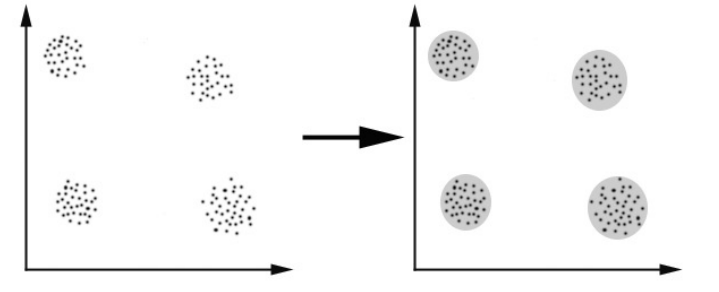
\includegraphics[width=.6\textwidth]{img/chapter-3/Clustering.png}
\caption{Esempio di clustering}\label{img:clustering}
\end{figure}

Per effettuare il clustering, generalmente, si eseguono i seguenti passaggi:
\begin{enumerate}
    \item Prendere un insieme di istanze appartenenti al workload (o ad una sua trasformazione mediante PCA)
    \item Scegliere i parametri del workload da considerare per effettuare la clusterizzazione (omettere i parametri che portano una quantità di varianza bassa)
    \item Selezionare una metrica di distanza (utile per la valutazione della similarità tra le istanze)
    \item Trattazione degli outliers (dati che sono molto distanti dagli altri, e che potrebbero falsare il risultato finale)
    \item Data scaling (utile per evitare che parametri con range di valori molto diversi tra di loro possano influenzare in maniera sproporzionata il risultato finale)
    \item Effettuare il clustering (utilizzando uno degli algoritmi di clustering esistenti)
    \item Interpretazione dei risultati (andare a valutare la qualità del clustering effettuato)
    \item Cambiare i parametri e/o il numero di cluster e ripetere i passi dal 3 al 7
    \item Selezionare un componente rappresentativo per ogni cluster
\end{enumerate}

\begin{warn}
Negli appunti si fa utilizzo del termine \textbf{istanza}, che per il seguente ambito è sinonimo di \textbf{componente}. Tale termine viene utilizzato per indicare un'entità del workload che viene caratterizzata da un insieme di parametri.
\end{warn}

\subsubsection{Campionamento delle componenti}
Il \textbf{Campionamento delle istanze} è una tecnica che va a selezionare un sottoinsieme di componenti del workload prima di proseguire nell'algoritmo di clustering. Ciò è dovuto al fatto che gli algoritmi di clustering sono computazionalmente costosi, e pertanto si cerca di ridurre la quantità di dati da considerare. La tecnica di selezione delle componenti da andare a considerare può essere di varia natura. Precisamente si studiano (per il seguente corso), le seguenti tecniche:
\begin{itemize}
    \item \textbf{Random Sampling}: Si va a selezionare un sottoinsieme di componenti in maniera casuale
    \item \textbf{Resource Consuption Based Sampling}: Si va a selezionare un sottoinsieme di componenti in base alla quantità di risorse che esse consumano (si vanno a selezionare le componenti che consumano più risorse)
\end{itemize}

Per capire se ho effettuato un buon campionamento, una volta effettuato il clustering vado a vedere, sul workload intero, se posso associare le componenti mancanti ai cluster trovati. Se il numero di componenti non assignabili è alto allora è indice di un cattivo campionamento.

\subsubsection{Selezione dei parametri}
Vado a selezionare un sottoinsieme di parametri rtappresentativi delle componenti. Tali parametri devono essere scelti in maniera tale che siano in grado di rappresentare la maggior quantità di varianza possibile o rispetto all'impatto sulle performance. Per fare ciò si può utilizzare la PCA, andando a selezionare i parametri che portano più varianza. Facendo in questo modo introduco una quantità di varianza persa a discapito, però, della riduzione della dimensionalità del problema, e di conseguenza, della riduzione del tempo speso per effettuare la clusterizzazione.

\subsubsection{Metrica di distanza}
Una metrica di distanza mi permette di calcolare la ditanza tra varie componenti in spazi n-dimensionali, dove n è il numero di parametri considerati. Le metriche più utilizzate sono:
\begin{enumerate}
    \item \textbf{Distanza Euclidea}: La distanza euclidea è la distanza più intuitiva, ed è definita come:
    \[d(X_i,X_j) = \sqrt{\sum_{k=1}^{n}(X_{ik} - X_{jk})^2}\]
    Dove \(X_i\) e \(X_j\) sono due punti nello spazio n-dimensionale, e \(X_{ik}\) e \(X_{jk}\) sono le loro coordinate(tale distanza è applicabile solo in spazi reali, quindi a parametri reali. Oltretutto la distanza euclidea utilizza il principio introdotto dal teorema di Pitagora [il teorema di Pitagora è un eccezione della formula precedente, precisamente solo per spazi bidimensionali]).
    Nonostante la distanza euclidea sia applicabile solo ad insiemi di parametri reali, essa è la più utilizzata, sopratutto per la sua similarità con la deviazione standard (guardare l'espessione matematica delle due grandezze)

    \item \textbf{Distanza Euclidea Pesata}: La distanza euclidea pesata è una variante della distanza euclidea che permette di andare a pesare i vari parametri in base alla loro importanza. La formula è la seguente:
    \[d(X_i,X_j) = \sqrt{\sum_{k=1}^{n}a_k(X_{ik} - X_{jk})^2}\]
    Dove \(a_k\) è il peso associato al parametro \(k\). Tale distanza è utile quando si vuole dare più importanza ad alcuni parametri rispetto ad altri. Tale metrica è utilizzata spesso o quando i parametri non sono stati scalati o quando i parametri hanno livelli di importanza diversi.

    \item \textbf{Distanza Euclidea Quadrata}: La distanza euclidea quadrata è una variante della distanza euclidea che evita di dover calcolare la radice quadrata, dato che tale operazione è computazionalmente costosa. La formula è la seguente:
    \[d(X_i,X_j) = \sum_{k=1}^{n}(X_{ik} - X_{jk})^2\]
    Tale distanza è utile quando si vuole evitare di effettuare la radice quadrata, dato che non cambia l'ordinamento delle distanze tra i punti. Tale metrica cerca di enfatizzare i valori più distanti (rendend distanze grandi ancora più grandi), e favorendo quelle piccole (rendendo distanze piccole ancora più piccole).
    
    \item \textbf{Distanza di Chi-Quadrato (Chi-square distance)}: La distanza di Chi-Quadrato (Chi-square) è una metrica che viene utilizzata principalmente per dati categoriali. La formula è la seguente: 
    \[d(X_i,X_j) = \sum_{k=1}^{n}\frac{(X_{ik} - X_{jk})^2}{X_{ik} + X_{jk}}\]
    Tale distanza è utile quando si vuole dare più importanza ai parametri che hanno valori più piccoli, dato che la somma al denominatore rende tale distanza più sensibile a piccole differenze tra i valori piccoli. Tale metrica, però, può essere applicata solo a dati che sono compatibili numericamente o che almeno appartengono allo stesso ordine di grandezza (se si avessero valori che hanno differenze grandi, il peso associato alla loro differenza sarebbe molto piccolo, e quindi non verrebbe considerata).

    \item \textbf{Distanza di Hamming}: La distanza di Hamming è una metrica che viene utilizzata principalmente per dati categoriali. La formula è la seguente:
    \[d(X_i,X_j) = \sum_{k=1}^{n}\delta(X_{ik}, X_{jk})\]
    Dove \(\delta(X_{ik}, X_{jk})\) è una funzione che vale 1 se \(X_{ik} \neq X_{jk}\), altrimenti vale 0. Tale distanza è utile quando si vuole confrontare dati categoriali, dato che conta il numero di differenze tra i due vettori. Non è utile per dati numerici "continui", il che la rende difficilmente utilizzabile.

\end{enumerate}

\begin{info}
Tutto le tecniche precedentemente presentate rispettano la definizione base di metrica. Una metrica si può definire formalmente come:

Dato uno spazio \(S\), una funzione \(d: S \times S \rightarrow \mathbb{R}\) è una metrica se per ogni \(X_i, X_j, X_k \in S\) rispetta le seguenti proprietà:
\begin{itemize}
    \item \(d(X_i,X_j) \geq 0\) (Non negatività)
    \item \(d(X_i,X_j) = 0 \iff X_i = X_j\) (Identità degli indiscernibili)
    \item \(d(X_i,X_j) = d(X_j,X_i)\) (Simmetria)
    \item \(d(X_i,X_j) \leq d(X_i,X_k) + d(X_k,X_j)\) (Disuguaglianza triangolare)
\end{itemize}

\end{info}

\subsubsection{Trattazione degli outliers}
Gli \textbf{outliers} sono componenti del workload che sono molto distanti dalle altre componenti. La presenza di outliers può falsare il risultato finale del clustering, dato che tali componenti potrebbero essere considerate come cluster a se stanti, o potrebbero influenzare la posizione dei centroidi. Pertanto è utile andare a trattare gli outliers prima di effettuare il clustering. Le tecniche più utilizzate per trattare gli outliers sono:
\begin{itemize}
    \item \textbf{Rimozione degli outliers}: Si va a rimuovere le componenti che sono molto distanti dalle altre componenti. Tale tecnica è utile quando si vuole evitare che gli outliers influenzino il risultato finale del clustering. Il problema principale di tale tecnica è che si potrebbe andare a rimuovere componenti che sono effettivamente parte del workload, e che potrebbero essere importanti per la caratterizzazione del workload stesso.
    \item \textbf{Trasformazione degli outliers}: Si va a trasformare le componenti che sono molto distanti dalle altre componenti. Tale tecnica è utile quando si vuole evitare che gli outliers influenzino il risultato finale del clustering, senza però rimuovere componenti che potrebbero essere importanti per la caratterizzazione del workload stesso. La trasformazione più comune è la normalizzazione
\end{itemize}

\subsubsection{Data Scaling}
Il \textbf{Data Scaling} è una tecnica che permette di andare a scalare i parametri delle componenti, in maniera tale che tutti i parametri abbiano lo stesso peso nella valutazione della distanza tra le componenti, quindi i dati che vengono trattati sono trattati secondo una distribuzione normale e quindi confrontabili anche guardando le unità di misura. Ci sono varie tecniche di normalizzazione che si possono applicare ai dati. Precisamente quelle utilizzate in questo corso sono:
\begin{itemize}
\item \textbf{Normalizzare ad una distribuzione normale (Z-score normalization)}: Per il calcolo di tale normalezzazione, si utilizza la formula:
\[x^0_{ik} = \frac{x_{ik} - \overline{x_{k}}}{s_{k}}\]
Dove \(x_{ik}\) è il valore del parametro \(x\), \(\overline{x_{k}}\) è la media del parametro \(x\) e \(s_{x_s}\) è la deviazione standard del parametro \(x\). Tale tecnica permette di avere una distribuzione normale con media 0 e deviazione standard 1. Tale tecnica è molto efficiente quando i dati seguono una distribuzione normale.

\item \textbf{Pesata}: Si va a pesare i parametri in base alla loro importanza. La formula è la seguente:
\[x'_s = w_k * x_s\]
Dove \(w_k\) è il peso associato al parametro \(x\). Tale tecnica è utile quando si vuole dare più importanza ad alcuni parametri rispetto ad altri. \(w_k\) è un valore di peso relativo, e può essere calcolato anche mediante la formula: \(w_k=\frac{1}{s_k}\)

\item \textbf{Range Normalizzation}: La range normalizzation (o in altri campi assimilabile all'equalizzazione dell'istogramma) è una tecnica che permette di andare a scalare i parametri in un intervallo specifico. Per comprendere meglio tale tecnica, si può vedere la formula come: 
\[
x'_{ik} = \frac{x_{ik} - min(x_k)}{max(x_k) - min(x_k)}
\]
Il problema associato a tale tecnica di scaling è che è molto e fortemente influenzata dagli outliers, dato che tali valori andranno a definire il range di valori

\item \textbf{Percentile Normalization}: La percentile normalization è una tecnica che permette di andare a scalare i parametri in base ai percentili. Tale tecnica è utile quando si vuole evitare che gli outliers influenzino il risultato finale del clustering. La formula è la seguente:
\[
x'_{ik} = \frac{x_{ik} - x_{2.5k}}{x_{97.5k} - x_{2.5k}}
\]

Tale formula cerca di andare a valutare il "massimo" e "minimo" della Range Normalization utilizzando i percentili, rendendo il sistema più resistente agli outliers.
\end{itemize}

\subsection{Agglomerative Hierarchical Clustering}
Le tecniche di clustering sono diverse e possono suddividersi in due macro-categorie: quelle \textbf{gerarchiche} e quelle \textbf{Non Gerarchiche}. Le tecniche gerarchiche permettono di costruire un sistema di cluster annidati tra loro (in base al livello del cluster), mentre le tecniche  non gerarchiche cerca di non annidare in alcun modo i cluster. Nei nostri casi di studio la categoria di tecniche di clustering che ci interessa sono solo i clustering gerarchici agglomerativi (le tecniche di clustering gerarchico possono essere anche divisive, in base alla struttura della tecnica con cui si costruisce il sistema di cluster [\ref{img:clustering-graph}]).

\begin{figure}[h]
\centering
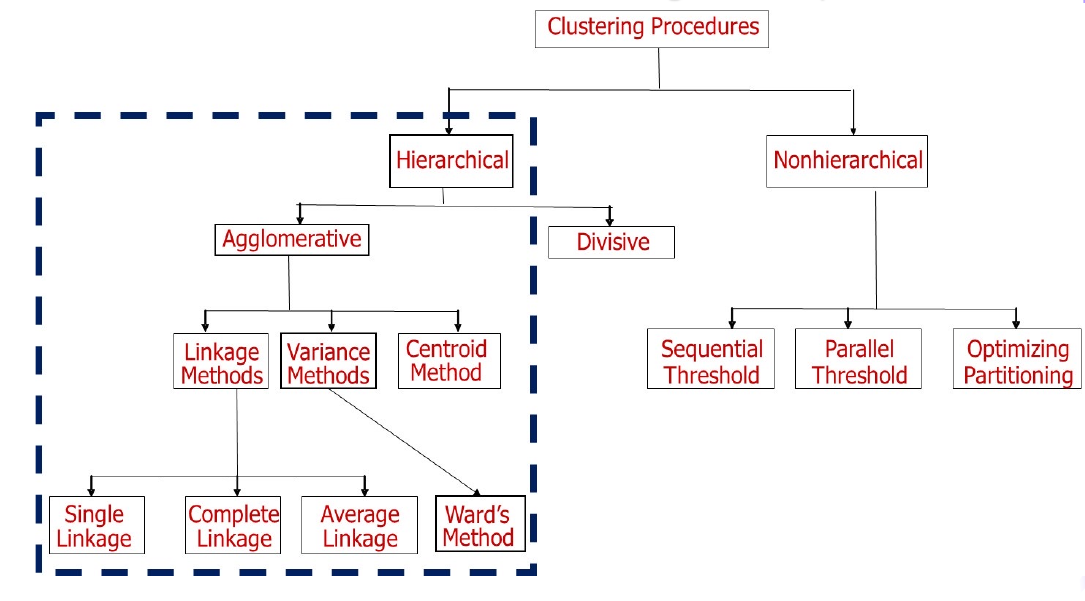
\includegraphics[width=.8\textwidth]{img/chapter-3/clustering-graph.png}
\caption{Esempio di clustering gerarchico}\label{img:clustering-graph}
\end{figure}

Fatta una paronamica generale sul clustering, ai fini del corso, andremo a concentrarci sul clustering gerarchico agglomerativo. Partendo dal considerare il \textbf{clustering gerarchico}, esso può essere di due tipi:
\begin{itemize}
    \item \textbf{Agglomerativo}: Si parte dall'avere un cluster per ogni componente, e poi si prosegue agglomerando i cluster fino a che non si ottiene un unico cluster
    \item \textbf{Divisivo}: Si parte da un cluster in cui sono contenutre tutte le compoenti e si prosegue dividendo i vari cluster secondo particolari metodi.
\end{itemize}

Il clustering \textbf{gerarchico agglomerativo} è una tipologia di clustering che parte dall'avere tanti cluster (uno per ogni componente), e poi si occupa di andare ad agglomerare tali cluster in base a particolari metriche. Tali metriche si basano su concetti differenti di definizione di similarità, e per ognuno ci sono varie considerazioni da fare. Le tecniche principali di clustering agglomerativo sono:
\begin{itemize}
    \item \textbf{Linkage Methods}: Vado a collegare i vari cluster in base alla metrica di distanza che vige tra di loro. Dato che non posso valutare la distanza di tutti i punti si può andare a considerare una metrica differente basandosi su diverse e particolari componenti del cluster:
    \begin{itemize}
        \item \textbf{Single Linkage}: Vado a definire la metrica di distanza tra due cluster come la più piccola distanza tra due punti dei cluster (la distanza dei punti più vicini tra due cluster) [\ref{img:single-linkage}]
        \item \textbf{Complete Linkage}: Vado a definire la metrica di distanza come la distanza maggiore tra due punti di un cluster [\ref{img:complete-linkage}]
        \item \textbf{Average Linkage}: Vado a definire la metrica di distanza come la distanza media dei punti tra due cluster [\ref{img:average-linkage}]
    \end{itemize}

    \item \textbf{Centroid Methods}: Molto simile ai metodi linkage, ma al postro di considerare le istanze direttamente appartenenti al cluster, si va a considerare il centroide del cluster (la media dei punti appartenenti al cluster) e si va a valutare la distanza tra i centroidi dei vari cluster (il centroide non è detto che faccia parte degli elementi del cluster)

    \item \textbf{Variance Methods}: Tale metodo cerca di minimizzare la varianza intra-cluster e cerca di massimizzare la varianza inter-cluster. L'utilizzo effettivo di tale metodo ricade nell'utilizzo del metodo di Ward, che cerca di minimizzare la somma delle varianze all'interno di ogni cluster. A livello formale quello che si va a fare è calcolare la distranza tra due cluster mediante l'utilizzo della distanza euclidea quadrata tra i centroidi dei due cluster, pesata per il numero di elementi che compongono i due cluster. La formula è la seguente:
    Dato il cluster \(P\) ed il cluster \(Q\), il calcolo della distanza mediante il \textbf{metodo di Ward} è:
    \[
    d(P,Q) = 2\frac{|P||Q|}{|P| + |Q|}||(\overline{x}_{P},\overline{x}_{Q})||^2
    \]
    Dove \(|P|\) e \(|Q|\) sono il numero di elementi che compongono i cluster \(P\) e \(Q\), mentre \(\overline{x}_{P}\) e \(\overline{x}_{Q}\) sono i centroidi dei cluster \(P\) e \(Q\).
\end{itemize}

\begin{figure}[h]
\centering
\begin{subfigure}[b]{0.8\textwidth}
\centering
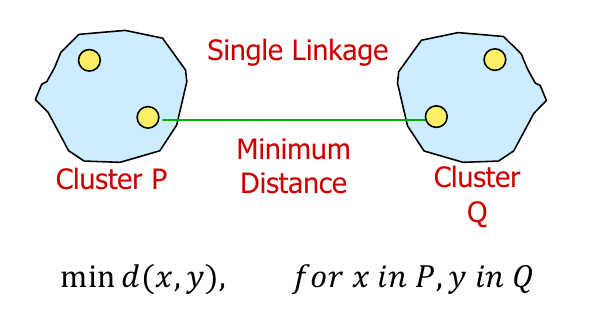
\includegraphics[width=\textwidth]{img/chapter-3/single-linkage.png}
\caption{Single Linkage}\label{img:single-linkage}
\end{subfigure}

\hfill

\begin{subfigure}[b]{0.8\textwidth}
\centering
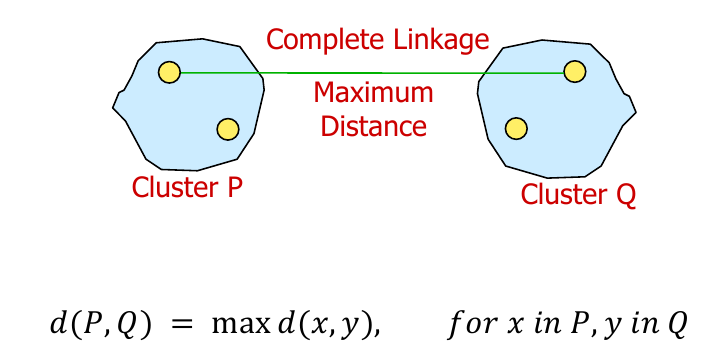
\includegraphics[width=\textwidth]{img/chapter-3/complete-linkage.png}
\caption{Complete Linkage}\label{img:complete-linkage}
\end{subfigure}

\hfill
\begin{subfigure}[b]{0.8\textwidth}
\centering
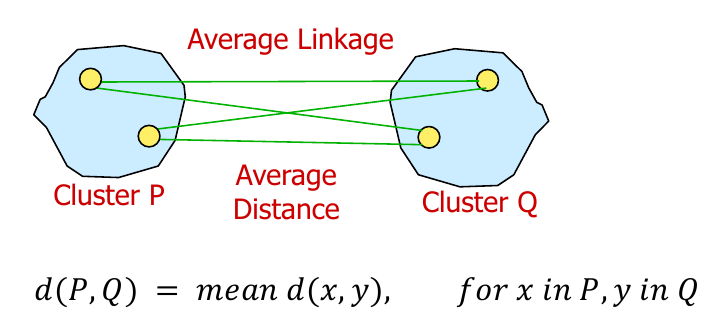
\includegraphics[width=\textwidth]{img/chapter-3/average-linkage.png}
\caption{Average Linkage}\label{img:average-linkage}
\end{subfigure}

\caption{Tipi di metriche per il Linkage Clustering}
\end{figure}

In generale, quindi, un algoritmo di clustering gerarchico agglomerativo segue i seguenti passi:

\begin{enumerate}
\item Calcolo della matrice di distanza tra tutte le componenti date in input
\item Impostare ogni componente come un cluster a se stante
\item Ripetere fino a che non rimane un solo cluster:
\begin{itemize}
    \item Trovare i due cluster più vicini secondo la metrica di distanza scelta ed unirli in un unico cluster
    \item Aggiornare la matrice di distanza per tenere conto del nuovo cluster
    \item Ripeti fino a che non rimane un solo cluster
\end{itemize}
\end{enumerate}
\clearpage

La parte in cui incidono di più le decisioni dei criteri di distanza (linkage, centroid, variance) è nella parte di calcolo della distanza dell'algoritmo. Ad ogni possibile metodo utilizzato, viene associato un diverso modo di calcolare la matrice di distanza, e di conseguenza, si avrà una diversa struttura del clustering finale.
La scelta su quali cluster agglomerare rimane la stessa, ovvero si agglomerano i cluster con la distanza minore tra loro. (questo accade per tutti i metodi, tale metodo di scelta di agglomerazione prescinde dalla metrica utilizzata per calcolare la distanza tra i cluster [che invece contiene una serie di criteri di scelta precedentemente discussi]).

La parte più importante di un clustering gerarchico è il fatto che poi alla fine si va a ricavare un legame tra i vari cluster, che può essere rappresentato mediante un dendogramma. Un dendogramma è un grafo aciclico orientato, dove il nodo rappresenta il cluster "finale" (intero dataset), le foglie sono i singoli elementi, ed i nodi, sono i cluster che nel processo sono stati agglomerati. La comodità di avere un dendogramma è che si può andare a "tagliare" il grafo ad un certo livello, ottenendo così un numero di cluster desiderato. (guardare figura [\ref{img:dendogramma}]). Quado vado a scegliere il livello a cui tagliare il dendogramma, mediante la larghezza del dendogramma, riesco a capire se due cluster se hanno una varianza più bassa o più alta. Più sono vicino alla radice, meno sono i cluster, ma la similarità intra-cluster si riduce. Mentre, più sono vicino alle foglie, più sono i cluster, e la similarità intra-cluster aumenta. 

\begin{figure}[h]
\centering
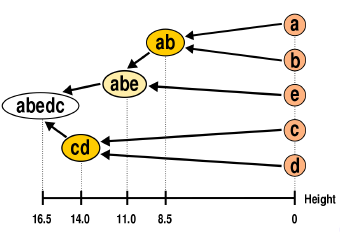
\includegraphics[width=.8\textwidth]{img/chapter-3/dendogramma.png}
\caption{Esempio di dendogramma}\label{img:dendogramma}
\end{figure}

\begin{warn}
In base al metodo utilizzato si avrà una clusterizzazione differente. Quindi la scelta del metodo di calcolo della distanza è fondamentale per ottenere un buon risultato finale.
\end{warn}

\subsubsection{Interpretazione del clustering}
Alla fine del clustering, tutte le componenti facenti parte dell'insieme di dati in ingresso sono associati ad un singolo cluster. In generale posso eliminare i cluster poco influenti (che occupano poche risorse) e che hanno una dimensione molto piccola (poche componenti) [Attenzione, le regole precedentemente presentate per la selezione di un cluster non possono essere divisie, devono essere entrambe vere, altrimenti si potrebbe ricadere in errori di valutazione]. Ottenuti i cluster, si cerca di interpretarli in maniera funzionale (in baso alla tipologia di dato che si sta andando a valutare).

Una volta ottenuti e valutati i cluster si va a trovare un singolo valore rappresentativo per ogni cluster, ciò ci permetterà di poter rappresentare il workload mediante un minor numero di componenti.

I cluster tra loro devono essere quanto più dissimili possibile, mentre le componenti all'interno di un cluster devono essere quanto più simili possibile tra di loro. In statistica possiamo definire tale concetto parlando di varianza; più precisamente si enuncia che:
\textit{La varianza intra-cluster dev'essere quanto più piccola possibile, mentre la varianza inter-cluster dev'essere quanto più grande possibile.}
L'unico problema legato all'utilizzo della varianza è che non rispetta la disuguaglianza triangolare, e pertanto non può essere utilizzata come metrica di distanza per il clustering. Pertanto si utilizza la devianza come metrica per valutare la bontà del clustering effettuato, questo perchè rispetta la disuguaglianza triangolare:
\[
devianza\_totale = devianza\_intra\_cluster + devianza\_inter\_cluster
\label{for:triangolare}
\]

In maniera più formale, ci è richiesto un metodo per valutare tali devianze. Per valutare la devianza intra-cluster si utilizza la seguente formula:

Dati \(n\) oggetti in uno spazio vettoriale \(d\)-dimensionale\\ \(X_i = (x_{i1}, x_{i2},\dots, x_{id})\), \(\forall i \in [1,n]\), si definisce devianza intra-cluster:

\[
intra\_cluster\_deviance = \sum_{k=1}^{K}\sum_{i=1}^{n_k}||X_i - \overline{X}_k||^2
\]

Dove:
\begin{itemize}
\item \(\overline{X}_k = \frac{1}{n_k}\sum_{C(i)=k}X_i\): Centroide del cluster \(k\)
\item \(n_k\): Numero di oggetti nel cluster \(k\)
\item \(||X_i - X_j||^2 = \sum_{p=1}^{d}(x_{ip} - x_{jp})^2\)
\item \(K\): Numero di cluster che si vanno a considerare
\end{itemize}

Mentre per valutare la devianza inter-cluster si utilizza la seguente formula:

Dati i \(K\) cluster e \(\overline{X}\) media di tutti gli elementi. Si definisce la devianza inter-cluster come:
\[
inter\_cluster\_deviance = \sum_{k=1}^{K}n_k||\overline{X}_k - \overline{X}||^2
\]

Dove (formalmente):
\begin{itemize}
\item \(\overline{X} = \frac{1}{n}\sum_{i=1}^{n}X_i\): Media di tutte le componenti date in ingresso all'algoritmo
\item \(n\): il numero di componenti dati in ingresso all'algoritmo
\end{itemize}

Si può dimostrare che la varianza intra-cluster e la varianza inter-cluster rispettano la disuguaglianza triangolare (vedi formula [\ref{for:triangolare}])

\subsection{Valutazione della devianza persa}
Quando vado ad effettuare la sintetizzazione del workload mediante l'utilizzo di PCA + clustering, devo valutare la quantità di devianza persa. La devianza persa è la quantità di devianza che non viene più rappresentata dalle componenti selezionate per rappresentare il workload. Per calcolarla, vado a valutare i seguenti valori:
\begin{itemize}
    \item \textbf{Varianza persa PCA}: La devianza portata dai parametri che non sono stati selezionati dopo la PCA
    \item \textbf{Varianza persa Clustering}: La devianza intra-cluster, ovvero la devianza che non viene più rappresentata dalle componenti selezionate per rappresentare il workload
\end{itemize}

Per il calcolo della devianza totale persa vado a considerare la seguente formula:
\[
devianza\_persa = devianza\_persa\_PCA + (devianza\_guadagnata\_PCA * devianza\_intra\_cluster)
\]

Oppure in maniera identica posso utilizzare la formula:
\[
devianza\_persa = 1 - (devianza\_guadagnata\_PCA * devianza\_inter\_cluster)
\]

In questo secondo caso sono andato a valutare prima la quantità effettiva di varianza "guadagnata" tra i due processi e poi ho sottratto ad 1 (essendo tutto espresso in percentuali).

Esempio:\\
Una volta effettuata la PCA con la selezione dei parametri sul mio workload ho che la devianza considerata è del \(95\%\).\\
Poi facendo il clustering, scopro che la mia devianza intra-cluster è pari al \(10\%\) e di conseguenza quella inter-cluster è pari al \(95\%\).\\
Di conseguenza posso calcolare la devianza totale persa come:
\[
devianza\_persa = devianza\_persa\_PCA + (devianza\_guadagnata\_PCA * devianza\_intra\_cluster)=
\]
\[
= 0.05 + (0.95 * 0.10) = 0.145 = 14.5\%
\]

Se vado a calcolare tale valore con l'altra formula, ottengo:
\[
devianza\_persa = 1 - (devianza\_guadagnata\_PCA * devianza\_inter\_cluster)=
\]
\[
= 1 - (0.95 * 0.90) = 1 - 0.855 = 0.145 = 14.5\%
\]

Notiamo come i due valori siano esarramente uguali.

\begin{info}
\textit{Tale dimostrazione è stata aggiunta solo a scopo didattico e non è richiesta ai fini dell'esame}
Il collegamento tra i due calcoli è molto semplice e risulta dimostrabile. Per dimostrare tale collegamento si può procedere nel seguente modo (consideriamo la deviazione guadagnata dalla pca denotata come dgp, mentre la deviazione persa dalla pca dpp, mentre poi vado a considerare la deviazione intra-cluster come dic, mentre la deviazione inter-cluster dec). Posso dimostrare tale legame nel seguente modo:
\[
deviazione\_persa = dpp + (dgp * dic) = 1 - dgp + (dgp * dic)=
\]
\[
= 1 - (1 - dic) * dgp = 1 - dec * dgp
\]
Come possiamo vedere alla fine siamo arrivati alla seconda forma di calcolo della devianza persa totale
\end{info}

\subsection{Modelli di Markov}
Un \textbf{modello di Markov} è una tipologia di modello in cui uno stato successivo o prossimo, dipende solamente dallo stato corrente. Esso può essere rappresentato, quindi, mediante l'utilizzo di un grafo. Un modello di markov, quindi, ha un modo di decidere il prossimo stato (che dipenderà solo da quello attuale). La possibilità di raggiungere un dato stato considerato lo stato precendente viene chiamata \textbf{Probabilità di transizione}, mentre la tabella con tutte le probabilità di raggiungere uno stato dato lo stato corrente, è detta \textbf{Matrice delle transizioni} (in inglese sarebbe matrice di transizione, ma tale definizione collide con le conoscenze precedenti di algebra e geometria). Tale tipologia di modello permette di trovare dei "pattern" o path, che vengono seguiti durante "l'utilizzo" di un applicativo (workload). Permettendo di andare a stressare il sistema su quelle operazioni che si sanno sono più ripetute (probabili). La stima della tabella delle transizioni è fatta tramite un'approccio di tipo frequentista

